% --- Documentclass specifications ---
\documentclass[italian]{tktltiki2}
\linespread{1.3}

% --- General packages ---
\usepackage[utf8]{inputenc}
\usepackage[T1]{fontenc}
\usepackage{lmodern}
\usepackage{epigraph}
\usepackage{microtype}
\usepackage{amsfonts,amsmath,amssymb,amsthm,booktabs,color,enumitem,graphicx}
\usepackage[pdftex,hidelinks]{hyperref}
% setting C language style listing
\usepackage{listings}
\lstset{
  language=C,
  basicstyle=\fontsize{8}{11}\selectfont\ttfamily
}
% Automatically set the PDF metadata fields
\makeatletter
\AtBeginDocument{\hypersetup{pdftitle = {\@title}, pdfauthor = {\@author}}}
\makeatother

% --- Language-related settings ---
\usepackage[fixlanguage]{babelbib}
% add bibliography to the table of contents
\usepackage[nottoc]{tocbibind}


% --- tktltiki2 options ---
%
% The following commands define the information used to generate title and
% abstract pages. The following entries should be always specified:
\title{%
  \huge Project Heimdall \\
  \large Proposta di implementazione per un web switch \\ 
    concorrente two-way di livello 7 (OSI) con \\
    politiche di bilanciamento del carico stateless e stateful
  }
\author{\emph{Alessio Moretti} - 0187698 \\\emph{Andrea Cerra} - 0167043\\\emph{Claudio Pastorini} - 0186256}
\date{\today}
\level{Corso di Ingegneria di Internet e del Web - A.A. 2014/2015}
\university{\textbf{Università di Tor Vergata}}
\department{\textbf{Ingegneria Informatica}}
\city{Roma}

% If the automatic page number counting is not working as desired in your case,
% uncomment the following to manually set the number of pages displayed in the abstract page:
%
% \numberofpagesinformation{16 pages + 10 appendix pages}

%


\begin{document}

% --- Front matter ---
\maketitle        % title page

\tableofcontents  % table of contents
\pagenumbering{gobble}

% --- Main matter ---
\mainmatter       % clear page, start arabic page numbering

\section{Example section}
% Example of a quote
\begin{quote}
\flushright
	\emph{Yggdrasil, l'albero del mondo, che congiunge i nove regni del cosmo con Asgard, la dimora degli dei.} \\ Heimdall, custode del Bifröst
\end{quote}

% Write some science here
Sample text and a reference\cite{lamport94}. Lorem ipsum dolor sit amet, consectetur adipiscing elit. Donec at lorem varius, sodales diam semper, congue dui. Integer porttitor felis eu tempor tempor. Proin molestie maximus augue in facilisis. Phasellus eros dui, blandit eu nibh ut, pharetra porta enim. Cum sociis natoque penatibus et magnis dis parturient montes, nascetur ridiculus mus. Aliquam ullamcorper risus pretium est elementum, eget egestas lorem fermentum. Etiam auctor nisi purus, vitae scelerisque augue vehicula sed. Ut eu laoreet ex. Mauris eu mi a tortor gravida cursus eget sit amet ligula.

\begin{figure}
\centering

\includegraphics[width=\textwidth]{images/thor}
\caption{Thor di Asgard, \emph{figlio di Odino}}
\end{figure}



\newpage
\section{Introduzione}

\subsection{Perchè Heimdall?}
Heimdall è il personaggio dell'universo Marvel, ispirato all'omonimo dio della mitologia norrena, egli è il guardiano del regno di Asgard e del Bifröst. Quest'ultimo è il ponte che unisce la Terra alla dimora degli dei ed Heimdall, come suo custode, ha il compito di aprirlo ed indirizzarlo verso gli altri mondo, permettendo solamente a chi è degno di attraversare le distese dello spazio. \\
Ci piace pensare che questo sia un po' il ruolo del software nato dal nostro progetto: che sia in grado di scegliere come meglio indirizzare le connessioni in arrivo, ponendosi come 'guardiano' di un cluster di server che fa ad esso capo. Quindi un \textbf{web switch} che sia funzionale sia per ricevere o trasmettere pacchetti di un regolare traffico HTTP che per bilanciare il carico dello stesso traffico in arrivo sulle varie macchine.

\subsection{Web switch di livello 7}
Nella terminologia delle reti informatiche uno \textbf{switch} è un commutatore a livello datalink, ovvero un dispositivo che si occupa di instradare opportunamente, attraverso le reti LAN, selezionando i frame ricevuti e reindirizzandoli verso la macchina appropriata a seconda di una propria tabella di inoltro. Un \textbf{web switch}, a livello applicativo, è capace di reindirizzare i dati in funzione dei pacchetti che riceve, analizzandone il contenuto e decidendo opportunamente la destinazione, occupandosi allo stesso tempo di reinoltrare anche l'eventuale risposta della macchina selezionata verso il client che l'ha generata. \\
Le applicazioni sono molteplici per l'implementazione a livello applicativo: può essere considerato un \textbf{proxy}, oppure, selezionando opportunamente la macchina con più velocità di risposta o con minore pressione, può agire come \textbf{bilanciatore di carico}. Infatti ognuno dei client che fa richiesta, ad esempio, per uno specifico sito web, invia un pacchetto ad un indirizzo IP pubblico che corrisponde a quello del nostro switch applicativo. Questi, dopo aver correttamente letto il pacchetto, si occupa di consultare una tabella di inoltro generata con una determinata \textbf{politica di scheduling} e quindi gestire l'inoltro della richiesta ed il reinoltro della risposta del webserver. tutto questo in maniera totalmente trasparente al client, qualsiasi sia la macchina che ha effettivamente risposto, che sia un web server oppure un cluster di macchine associate ad un ulteriore switch.

\begin{figure}
\centering
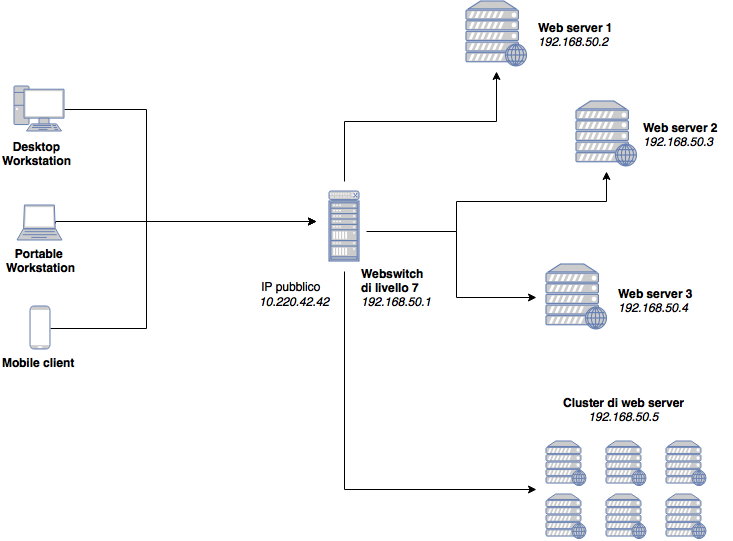
\includegraphics[width=\textwidth]{images/switch7}
\caption{Esempio di uno \emph{switch di livello 7 (OSI)}}
\end{figure}


\newpage
\section{Architettura}

\subsection{Server in ascolto}
\subsubsection{File di configurazione}
\subsubsection{Logging}
\subsubsection{Gestione degli errori}

\subsection{Pool manager}

\subsection{Scheduler}

\subsection{Worker}
\subsubsection{Gestione delle richieste}
\subsubsection*{Coda delle richieste}
\subsubsection*{Chunk di dati}
\subsubsection{Gestione delle connessioni}
\subsubsection*{Connessione}
\subsubsection*{Richieste HTTP}
\subsubsection*{Risposte HTTP}
\subsubsection{Thread di lettura}
\subsubsection{Thread di scrittura}
\subsubsection{Thread di richiesta}
\subsubsection{Thread di watchdog}

\newpage
\section{Ulteriori proposte}

\newpage
\section{Politiche di scheduling}
La schedulazione permette la selezione della macchina predisposta a rispondere alla richiesta HTTP appena arrivata da parte del client, si basa su una tecnica nota come \textbf{bilanciamento del carico}, ovvero la distribuzione del carico, solitamente di elaborazione o di erogazione di uno specifico servizio, tra più server. Questo permette di poter \textbf{scalare} sulla potenza di calcolo del cluster dietro al web switch, lasciando che siano diverse macchine a rispondere a seconda di quella che è più veloce, più performante, oppure monitorando costantemente lo stato dei server e scegliendo quello meno sottoposto ad una pressione del carico di lavoro. \\ \\ 
Nella nostra implementazione \textbf{thread scheduler} si occupa di fornire,  ogni volta che viene invocato, una macchina selezionata secondo una delle due politiche che andremo ora a spiegare nel dettaglio più avanti.


\begin{figure}[b]
\centering
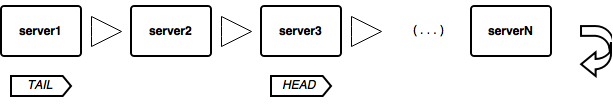
\includegraphics[width=\textwidth]{images/rrobin_stateless}
\caption{Schema di funzionamento del buffer circolare \label{fig: rrobin_sl}}
\end{figure}

\subsection{State-less: implementazione con Round-Robin}
L'algoritmo di scheduling Round-Robin (da adesso RR, \emph{n.d.r.}) è un algoritmo che agisce con prelazione distribuendo in maniera equa il lavoro, secondo una metrica stabilita in partenza. \\
L'algoritmo funziona utilizzando un buffer circolare come possiamo vedere in \emph{figura \ref{fig: rrobin_sl}}: questo permette di iterare la selezione su una lista di elementi precedentemente caricata. E' necessario quindi specificare due passi per il corretto funzionamento, dopo aver dato un rapido sguardo alla struttura che lo rappresenta nella nostra implementazione.\\\\
\begin{lstlisting}
typedef struct circular_buffer {
    Server      *buffer;
    int         buffer_position;
    int         buffer_len;
    
    Server      *head;
    Server      *tail;

    pthread_mutex_t mutex;

    ThrowablePtr (*allocate_buffer)(CircularPtr *circular, Server **servers, int len);
    ThrowablePtr (*acquire)(struct circular_buffer *circular);
    ThrowablePtr (*release)(struct circular_buffer *circular);
    void         (*progress)(struct circular_buffer *circular);
    void         (*destroy_buffer)(struct circular_buffer *circular);
} Circular, *CircularPtr;
\end{lstlisting}


\textbf{Inizializzazione del buffer:} in questa fase la struttura dati che rappresenta il buffer circolare, che mantiene due puntatori di \emph{testa} e \emph{coda}, viene inizializzata associandovi un array di puntatori di strutture di tipo \emph{Server} e viene eseguita la seguente funzione:
\begin{lstlisting}
    /* inside allocate_buffer ... */
    // allocating the buffer
    circular->buffer = *servers;
    circular->buffer_len = len;
    // setting params
    circular->head = circular->buffer;
    circular->tail = circular->buffer + (len - 1);
\end{lstlisting}
In un'ottica di \emph{produttore vs consumatore}

\subsection{State-aware: implementazione con monitor di carico}
\subsubsection{Modulo ApacheStatus}


\newpage
\section{Performance}
\subsection{Test di carico}
\subsection{Comparazione con Apache}
\newpage
\section{Future implementazioni}
\subsection{Analisi della richiesta}
\subsection{Webserver performante}


% --- References ---  
%
% bibtex is used to generate the bibliography. The babplain style
% will generate numeric references (e.g. [1]) appropriate for theoretical
% computer science. If you need alphanumeric references (e.g [Tur90]), use
%
% \bibliographystyle{babalpha-lf}
%
% instead.


\newpage
%\bibliographystyle{babplain-lf}
%\bibliography{references}
\renewcommand{\refname}{\normalfont\selectfont\normalsize\textbf{Annotazioni}} 
\begin{thebibliography}{9}
\bibitem{lamport94}
  Leslie Lamport,
  \emph{\LaTeX: a document preparation system},
  Addison Wesley, Massachusetts,
  2nd edition,
  1994.
  
\end{thebibliography}

% --- Appendices --- 
\newpage
\appendix
 
\section{Manuale per l'uso}

\section{Vagrant}

\section{Cluster virtuale}

\section{Tool per i debug}
\subsection{GDB}
\subsection{Valgrind}

\section{Tool per i test}
\subsection{PostMan}
\subsection{Telnet}
\subsection{HttPerf}
\subsection{Browser}

\end{document}